\documentclass[10pt]{article}

\usepackage[margin=0.82in]{geometry}
\usepackage[T1]{fontenc}
\usepackage{lmodern}
\usepackage{microtype}
\usepackage{amsmath,amssymb}
\usepackage{booktabs}
\usepackage{array}
\usepackage{enumitem}
\usepackage{xcolor}
\usepackage{url}
\usepackage{hyperref}
\usepackage{cleveref}
\usepackage{tikz}
\usetikzlibrary{arrows.meta,positioning,shapes.misc}

\definecolor{deepblue}{HTML}{17365D}
\definecolor{safegray}{HTML}{F2F4F7}
\definecolor{badred}{HTML}{9C2F2F}
\definecolor{goodgreen}{HTML}{176B43}
\hypersetup{
  colorlinks=true,
  linkcolor=deepblue,
  citecolor=deepblue,
  urlcolor=deepblue,
  pdftitle={Predicates, Not Assumptions},
  pdfsubject={A soundness and matched-baseline audit of LLM-guided IC3IA}
}

\setlist{nosep,leftmargin=*}
\setlength{\tabcolsep}{5pt}
\renewcommand{\arraystretch}{1.12}
\newcommand{\tool}{\textsc{Pono-LLM}}
\newcommand{\pono}{\textsc{Pono}}
\newcommand{\icthreeia}{\textsc{IC3IA}}
\newcommand{\btor}{\textsc{BTOR2}}
\newcommand{\llm}{\textsc{LLM}}
\newcommand{\code}[1]{\texttt{#1}}
\newcommand{\unsat}{\textsc{unsat}}
\newcommand{\sat}{\textsc{sat}}
\newcommand{\unknown}{\textsc{unknown}}

\title{\textbf{Predicates, Not Assumptions:}\\
  A Soundness and Matched-Baseline Audit of LLM-Guided IC3IA}
\author{Pono-LLM Research Project\\
  \url{https://github.com/swear01/pono-llm}\\
  \small Archival Technical Report}
\date{Evidence frozen 14 July 2026; report packaged 18 July 2026}

\begin{document}
\maketitle

\begin{abstract}
Large language models can propose semantically plausible invariants, but the
formal meaning of how those formulas enter a verifier is decisive.  We report a
soundness and matched-baseline audit of an LLM-guided extension of
\icthreeia{} in the \pono{} SMT-based model checker.  The original system
inserted LLM-proposed mutex formulas as \btor{} constraints.  This
under-approximated the concrete transition system: the model checker proved a
model in which behaviors had been assumed away.  Independent certification on
the original models rejected all 32 checkable legacy proofs, and bounded
reachability found violations of 30 of 32 tested mutex formulas.

We replace assumption injection with initial \emph{predicate} injection.
Candidates enrich the implicit-abstraction vocabulary without changing the
concrete initial states, transition relation, constraints, or safety
properties.  A false candidate can increase proof cost, but cannot manufacture
a safety result by excluding concrete behaviors.  We then re-evaluate the
apparent gains using original-model C1/C2/C3 certification, frozen candidate
replay, end-to-end cost accounting, and deterministic affine and quadratic
candidate generators of matched expressiveness.  On the corrected 21-task
set, LLM and deterministic quadratic candidates certify exactly the same seven
safe tasks; both corresponding portfolios reach eight safe and two unsafe
tasks.  A broader 1,919-file HWMCC census and a preregistered paired
source/lifted/raw representation gate likewise leave no defensible
LLM-specific solved-set or search-efficiency advantage.

The result is not a coverage-improvement claim.  It is an empirical
falsification and evaluation-methodology result: apparent LLM gains can arise
from an unsound trust boundary, an expressiveness-mismatched baseline, or
best-run accounting.  The repository releases the sound integration,
independent checkers, frozen artifacts, machine-readable claim ledger, and
explicit not-run decisions.
\end{abstract}

\section{Introduction}

IC3/PDR proves safety by constructing an inductive strengthening rather than
explicitly unrolling the transition relation~\cite{Bradley2011IC3}.
\icthreeia{} extends this idea to richer theories through implicit predicate
abstraction~\cite{Cimatti2014IC3IA}, and \pono{} provides a flexible
SMT-based implementation and research platform~\cite{Mann2021Pono}.  These
techniques still depend critically on finding useful predicates and
generalizations.  An LLM appears attractive here: source-like state names and
recurrence patterns can survive compilation into word-level \btor{}, while a
language model can propose relations such as counter bounds, accumulator
equalities, or polynomial recurrences.

The central danger is that a plausible formula is not evidence that the
formula is true.  A verifier integration must therefore answer two separate
questions:
\begin{enumerate}
  \item How may an untrusted proposal guide proof search without changing the
        concrete verification problem?
  \item After sound integration, what improvement is attributable to the LLM
        rather than to the candidate language or additional search budget?
\end{enumerate}

This project began with apparently strong positive results and ended with a
negative marginal-value result.  The reversal is scientifically useful because
each stage identifies a concrete evaluation failure mode.  First, LLM mutex
hints had been encoded as assumptions, making the reported safety results
unsound for the original models.  Second, after replacing assumptions with
sound abstraction predicates, the remaining ``LLM-only'' examples were only
unique relative to verifier engines, not relative to deterministic generators
of the same affine and quadratic forms.  Third, broader and preregistered gates
did not recover a source-representation, phase, grammar-routing, or compactness
advantage.

The contributions of this report are:
\begin{itemize}
  \item an original-model audit that rejects 32/32 checkable legacy proofs and
        directly demonstrates the danger of converting semantic hints into
        concrete assumptions;
  \item a sound initial-predicate interface for \icthreeia{} in which arbitrary
        candidates refine the abstraction vocabulary but do not restrict the
        concrete model;
  \item independent bit-vector C1/C2/C3 checkers, every-property handling,
        exact Houdini filtering, frozen replay, and explicit \unknown{}
        semantics;
  \item a matched-baseline evaluation showing that deterministic affine and
        quadratic candidate generators cover every current LLM solve;
  \item a sequence of broader, preregistered population and mechanism gates
        that records failures and \emph{not-run} outcomes without moving the
        success criteria after observing results.
\end{itemize}

Our scoped conclusion is deliberately narrower than ``LLMs do not help formal
verification.''  Under the models, candidate languages, budgets, and solver
configurations evaluated here, no defensible LLM-specific solved-set or
search-efficiency advantage survives soundness repair and matched deterministic
comparison.

\section{Background and Verification Semantics}
\label{sec:semantics}

\subsection{Transition systems and safety}

We model a word-level transition system as
\[
  M=(X,U,I(X),T(X,U,X'),C(X,U),\{B_j(X)\}_{j=1}^{m}),
\]
where $X$ are state variables, $U$ are inputs, $I$ is the initial-state
formula, $T$ is the transition relation, $C$ contains original model
constraints, and each $B_j$ is a bad-state property.  The evaluated tasks are
primarily software-origin bit-vector models in \btor{}, a typed word-level
transition-system format~\cite{Niemetz2018BTOR2}, drawn from Hardware Model
Checking Competition distributions~\cite{HWMCC}.

For a proposed invariant conjunction $H(X)$, an independent certificate
requires, under exact fixed-width bit-vector semantics,
\begin{align}
  \text{C1: }& I(X)\land C(X,U)\land\neg H(X) &&\text{is \unsat},\label{eq:c1}\\
  \text{C2: }& H(X)\land C\land T\land C'\land\neg H(X') &&\text{is \unsat},\label{eq:c2}\\
  \text{C3$_j$: }& H(X)\land C(X,U)\land B_j(X) &&\text{is \unsat}\label{eq:c3}
\end{align}
for every bad property $j$.  A satisfying query is a concrete refutation.
An SMT timeout or \unknown{} result is no evidence of induction.

\subsection{IC3IA predicate abstraction}

\icthreeia{} performs IC3 over Boolean labels corresponding to theory
predicates and incrementally refines an implicit abstraction.  For a concrete
predicate $p(X)$, the abstraction associates a Boolean label with $p(X)$ and a
next-state label with $p(X')$.  Adding a predicate partitions the concrete
state space more finely and strengthens the abstract relational transition
description, but a correct implicit abstraction remains an over-approximation:
every concrete transition has a corresponding abstract transition.  Therefore,
proving safety in the abstract model proves safety in the concrete model.

This distinction is subtle but essential.  Adding $p$ as abstraction
\emph{vocabulary} does not claim that $p$ is always true.  Both polarities may
occur in abstract states.  Adding $p$ as a concrete constraint instead removes
all executions in which $p$ is false.

\section{The Soundness Failure}
\label{sec:failure}

\subsection{Constraint injection is assumption injection}

The legacy path asked an LLM to identify pairs of Boolean-looking signals that
appeared mutually exclusive and encoded a hint $h(X)$, typically
$\neg(x\land y)$, as a \btor{} \code{constraint}.  Let the resulting model be
$M_h$.  Its reachable behaviors satisfy
\[
  \mathrm{Reach}(M_h)\subseteq\mathrm{Reach}(M).
\]
Consequently, $M_h$ safe does not imply $M$ safe.  If $h$ excludes a reachable
state needed by a counterexample, the model checker can soundly prove the
\emph{restricted} model while saying nothing about the original model.

\begin{figure}[t]
\centering
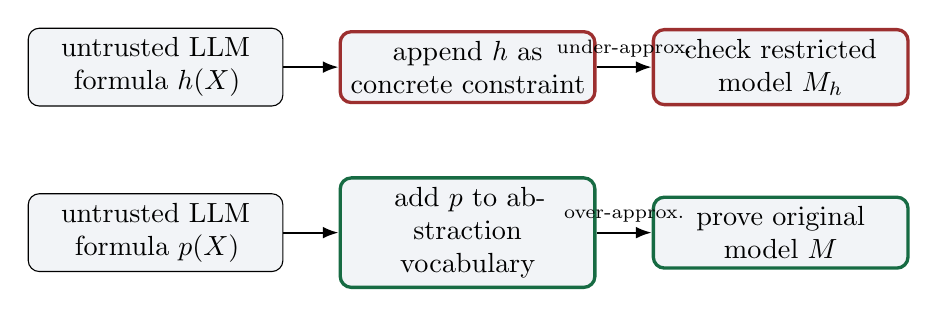
\begin{tikzpicture}[
  node distance=6mm and 7mm,
  box/.style={draw,rounded corners,align=center,minimum height=8mm,
              text width=30mm,fill=safegray},
  bad/.style={box,draw=badred,very thick},
  good/.style={box,draw=goodgreen,very thick},
  arr/.style={-{Latex[length=2mm]},thick}
]
  \node[box] (llm1) {untrusted LLM\\formula $h(X)$};
  \node[bad,right=of llm1] (assume) {append $h$ as\\concrete constraint};
  \node[bad,right=of assume] (restricted) {check restricted\\model $M_h$};
  \draw[arr] (llm1) -- (assume);
  \draw[arr] (assume) -- node[above,font=\scriptsize]{under-approx.} (restricted);

  \node[box,below=11mm of llm1] (llm2) {untrusted LLM\\formula $p(X)$};
  \node[good,right=of llm2] (pred) {add $p$ to abstraction\\vocabulary};
  \node[good,right=of pred] (original) {prove original\\model $M$};
  \draw[arr] (llm2) -- (pred);
  \draw[arr] (pred) -- node[above,font=\scriptsize]{over-approx.} (original);
\end{tikzpicture}
\caption{The old path assumed a candidate and restricted the concrete model.
The repaired path uses the candidate only to refine an over-approximate
abstraction; the safety verdict remains about the original model.}
\label{fig:trust}
\end{figure}

The error is a circular proof pattern: assume that a semantically suspicious
state never occurs, then conclude that it never occurs.  Source- or RTL-level
naming intuition is especially unreliable after bit-level compilation because
signals may represent encoded control, transient phases, or independent bits
rather than one-hot semantic states.

\subsection{Independent audit}

We built an exact Z3 bit-vector encoder for the supported \btor{} fragment and
checked the invariant returned by each legacy run against the original,
unmodified model using \cref{eq:c1,eq:c2,eq:c3}.  Of 32 independently
checkable old proofs, all 32 were rejected.  The dominant audit signature was
that the returned formula was inductive only in a way insufficient to establish
initial truth or safety on the original model.

A separate bounded-reachability scan tested the mutex hints themselves.  It
found a reachable state satisfying $x\land y$ for 30 of 32 tested pairs.  None
of the 32 was established as a true invariant.  The remaining two are not
counted as valid: absence of a bounded counterexample is not an inductive
proof.

These results invalidate the old proof count rather than merely weakening it.
The correct unit of evidence is an original-model certificate or a model-checker
verdict on the unchanged transition system, not \unsat{} after adding an
unproved assumption.

\section{Sound Predicate Injection}
\label{sec:repair}

The repaired interface is
\begin{center}
\code{pono -e ic3ia --initial-predicates predicates.json original.btor2}.
\end{center}
Each line contains a typed predicate AST.  Symbolic source-like names are
resolved to stable internal state references, and supported Boolean and
bit-vector operators are reconstructed in the \icthreeia{} solver.

During \code{IC3IA::initialize()}, the implementation calls the existing
\code{add\_predicate} path.  The method creates current and next abstraction
labels, links them to the concrete predicate evaluations, and asks the implicit
abstraction layer for a predicate-refinement constraint.  It does not append
the candidate to the concrete $I$, $T$, $C$, or $B_j$.  Thus the candidate can
be false on reachable states without creating a false safety result.

The precise soundness statement is:
\begin{quote}
Arbitrary candidate predicates may refine the abstraction vocabulary and
abstract transition relation while preserving an over-approximation of the
original transition system.  A reported safety result is therefore a proof of
the original unconstrained model, not an assertion that the candidates were
themselves invariants.
\end{quote}

This does \emph{not} imply that bad candidates are operationally harmless.
Each predicate adds an abstraction dimension and may increase SMT query size,
refinement count, memory use, or runtime.  Soundness and usefulness are
separate properties.

The implementation also provides two independent certification paths:
\begin{itemize}
  \item \code{scripts/cert\_check.py} parses a returned invariant and checks
        C1, C2, and every C3 obligation on the original model;
  \item \code{scripts/candidate\_cert\_check.py} checks a candidate conjunction
        directly and can apply exact Houdini elimination, removing candidates
        refuted by initial or one-step witnesses until a C1/C2-valid subset
        remains, then checking every bad property.
\end{itemize}
Unsupported forms and \unknown{} results are explicit.  No bounded-success
result is silently promoted to an invariant.

\section{Evaluation Protocol}
\label{sec:protocol}

The evaluation evolved into a falsification protocol designed to prevent four
common confounders.

\paragraph{Original-model proof.}
Every accepted safety result is either returned by a sound model-checker run on
the original \btor{} file or independently passes exact C1/C2/C3.  All bad
properties are checked.

\paragraph{Matched expressiveness.}
Verifier engines and candidate generators are separate baselines.  We compare
LLM candidates not only with plain induction, interpolation, and \icthreeia{},
but also with deterministic affine and quadratic template generators capable
of expressing the forms attributed to the LLM.

\paragraph{Frozen replay and total cost.}
Candidate capture is separated from proof replay.  Capture artifacts bind
benchmark, prompt, response, candidate, and metadata hashes.  Replay performs
no API call.  We distinguish proof-only time from
\[
  T_{\mathrm{end\text{-}to\text{-}end}}
  =T_{\mathrm{generation}}+T_{\mathrm{processing}}+T_{\mathrm{proof}}.
\]
Tokens and invalid outputs remain part of the record.

\paragraph{Preregistered gates.}
Later mechanism studies freeze their population, eligibility rules, success
thresholds, and stop conditions before observing the decisive outcome.  A
failed population prerequisite is recorded as \emph{not run}, not converted to
a smaller post-hoc experiment.

\begin{table}[t]
\centering
\caption{Evidence semantics used throughout the audit.}
\label{tab:evidence}
\small
\begin{tabular}{p{0.34\linewidth}p{0.58\linewidth}}
\toprule
Observation & Permitted interpretation \\
\midrule
LLM formula & Untrusted proposal only \\
Predicate accepted by IC3IA & Sound abstraction vocabulary; not a certified invariant \\
Bounded SAT witness & Refutes the candidate or establishes a bounded counterexample \\
Bounded UNSAT / timeout / SMT \unknown{} & No inductive conclusion \\
C1, C2, and all C3 queries \unsat{} & Certified inductive safety invariant \\
IC3IA \unsat{} on original model & Valid safety result for that model/configuration \\
\bottomrule
\end{tabular}
\end{table}

\section{Experimental Results}
\label{sec:results}

\subsection{Corrected 21-task comparison}

The first sound comparison appeared to leave three affine LLM-only examples:
\code{93.c}, \code{fib\_37}, and \code{fib\_05}.  They were unique only
relative to the tested \pono{} engines.  A deterministic affine generator
covered them once the formula language was matched.

Two nonlinear arithmetic cases, \code{fib\_23} and \code{fib\_30}, were then
used as a stronger reliability test.  Five independent captures for each case
produced a Houdini-certifiable conjunction in all ten captures.  This is a
positive reproducibility observation: the model repeatedly found an
appropriate nonlinear structure.  It is not an LLM-specific expressiveness
result, because a deterministic quadratic recurrence generator certifies both
cases as well.

\begin{table}[t]
\centering
\caption{Corrected full21 results.  Candidate columns count directly
certified safe tasks; portfolio columns add ordinary engine results.}
\label{tab:full21}
\small
\begin{tabular}{lrrr}
\toprule
Configuration & Certified safe & Portfolio safe & Portfolio unsafe \\
\midrule
LLM Houdini / engine+LLM & 7 & 8 & 2 \\
Deterministic quadratic / engine+det. & 7 & 8 & 2 \\
\midrule
LLM-specific after matching & \multicolumn{3}{c}{0} \\
\bottomrule
\end{tabular}
\end{table}

As shown in \cref{tab:full21}, the LLM and deterministic quadratic solved sets
are identical: seven candidate-certified safe tasks.  Adding the ordinary
engine portfolio gives both sides eight safe and two unsafe tasks.  The other
11 tasks remain unresolved under the recorded configurations.  Direct
certification itself is cheap on the nonlinear successes---median certificate
times are roughly 0.05--0.06 seconds---while median LLM generation is roughly
49 seconds for \code{fib\_23} and 126 seconds for \code{fib\_30}.  Therefore a
proof-only plot alone would badly misstate end-to-end cost.

\subsection{Broader HWMCC residual}

The broader gate structurally scanned 1,919 \btor{} files.  It identified 194
software-origin models, 89 non-array candidates, and 86 unique eligible models
after content deduplication.  Ordinary-engine and deterministic screens were
run before freezing 11 new deterministic-hard targets for LLM capture.

Across those targets, direct LLM Houdini certified none.  Raw predicate seeding
helped \icthreeia{} solve one model, \code{up.btor2}.  That result initially
looked like a useful abstraction-basis compactness observation, but it did not
survive stronger deterministic controls.  A 200-predicate static pool
reproduced the proof, and a fixed low-complexity relational ranker reproduced
it with a much smaller successful prefix.  In five matched replays, 15 LLM
predicates and 20 ranked predicates both solved 5/5; their median proof times
were 8.115 seconds and 2.134 seconds, respectively.  A ranked prefix of 15
failed while 16 succeeded, and the returned invariant at the successful
boundary independently passed C1/C2/C3.

The gate therefore contributes neither a new LLM-specific solve nor a
defensible compactness or runtime advantage.  It does illustrate a useful
distinction: a candidate set may help the abstraction even if the conjunction
is not itself inductive, but the source of that basis must still be compared
against deterministic alternatives.

\subsection{Paired representation, phase, and routing gate}

To test whether high-level representation rather than formula expressiveness
was the missing advantage, we constructed a paired source/target study.  The
population census contained 267 officially translated tasks, of which 164
were eligible.  A content- and family-independent 20-family pilot was frozen
before the LLM outcomes.  Each task was presented in three matched views:
source C, a target-derived lifted recurrence summary, and a raw \btor{}
property-cone sketch.

The LLM selected a strict grammar route rather than emitting unrestricted proof
text.  Deterministic code expanded the route into global or phase-conditioned
predicates, and the same original-target checker evaluated them.  Sixty calls
consumed 142,814 tokens and 229.16 seconds of recorded API latency; 36 routes
were valid and 24 invalid.

\begin{table}[t]
\centering
\caption{Decisions from the frozen paired representation gate.}
\label{tab:representation}
\small
\begin{tabular}{p{0.31\linewidth}p{0.20\linewidth}p{0.39\linewidth}}
\toprule
Hypothesis & Observation & Decision \\
\midrule
Source representation adds unique solve & Source/lifted/raw solve 1/1/2 baseline-hard tasks; source unique 0 & Rejected on pilot \\
Phase conditioning generalizes & One independent phase-only proof; threshold 3 & Threshold failed \\
LLM routing beats structural routing & Structural router covers the three-task LLM union & Rejected \\
Soundness of routed proofs & 12/12 routed \unsat{} rows certified; 0 unsafe false-safe & Supported \\
\bottomrule
\end{tabular}
\end{table}

The results in \cref{tab:representation} again separate correctness from
utility.  All 12 routed safety rows passed independent original-model
certification, and no unsafe control became safe.  Nevertheless, source had no
unique solve, phase conditioning added only one task against a threshold of
three, and the deterministic structural router covered the full three-task
union reached by all LLM representation arms.  Candidate-count reduction alone
did not become an end-to-end advantage after API latency and invalid routes.

\subsection{Reliability is not marginal value}

The LLM was not simply incapable of producing useful formulas.  Five-round
two-tier generation solved five known linear-solvable cases in 15/15 repeated
runs, and the two nonlinear cases produced certifiable candidate sets in 10/10
independent captures.  These observations matter for engineering: repeated
sampling can stabilize a demonstration.  They do not establish marginal
research value when a deterministic generator produces the same certified
forms at lower cost.  Reliability, coverage, uniqueness, and end-to-end utility
must be reported separately.

\section{Mechanism Gates and Scientific Stops}
\label{sec:stops}

Several later ideas were promising enough to preregister but did not produce a
utility experiment.  Reporting these outcomes prevents development controls or
near misses from being mistaken for evidence.

\paragraph{Modular algebraic certificates.}
A small kernel checks polynomial identities over $\mathbb{Z}/2^w\mathbb{Z}$
without unsound division or cancellation.  It validates development
certificates for \code{fib\_23} and \code{fib\_30}; a 20-case negative suite
rejects malformed, unsupported, false-initial, and unsafe cases at the expected
stages.  However, the frozen 267-task natural population contains zero task
eligible for the v1 contract: 39 require arrays, 221 have no supported
nonlinear update SCC, and the remaining seven have nonlinear SCCs exceeding
the frozen eight-branch cap.  Natural utility is therefore \emph{not run}, not
failed or supported.

\paragraph{Inductiveness-gap decomposition.}
Six frozen nonlinear candidates were tested to determine whether helpers,
deeper induction, or proof organization was the next bottleneck.  All six fail
C1 in an initial state, and exact Houdini removes every one during initial
filtering.  They are false conjectures, not valid invariants awaiting a better
proof graph.  Repairing them after inspecting the witnesses would be a new,
post-hoc experiment.

\paragraph{Known-map transport.}
A transport oracle was preregistered to move certified invariants through
affine state recoding, split/merge encoding, and input-latched stuttering
refinement.  The prerequisite census found 11 certified bases and six bases
applicable to the affine transformation, below frozen requirements of 12 and
eight.  The gate stopped before generating transformed variants, validating a
map, timing proof reuse, or calling an LLM.  Transport utility remains unknown.

These stops are part of the methodology.  Widening the operator language,
lowering 12/8 to 11/6, or adding hand-picked variants after seeing the census
would change the research question.  The repository records the development
capability separately from the absent confirmatory population.

\section{Discussion}

\subsection{Where the apparent advantage went}

The empirical trajectory admits a useful decomposition:
\begin{enumerate}
  \item \textbf{Assumption effect.}  The largest early gains came from removing
        concrete behaviors, not from better proof search.
  \item \textbf{Language effect.}  After sound integration, affine and
        quadratic formulas helped, but matched deterministic generators could
        instantiate the same language.
  \item \textbf{Sampling effect.}  More rounds improved hit rate and demo
        stability, not the set of formula families available to the proof.
  \item \textbf{Representation/routing effect.}  Source and phase information
        did not cross the frozen utility thresholds, and structural routing
        covered the LLM union.
  \item \textbf{Population effect.}  Two later proof mechanisms could not be
        evaluated on a sufficiently large independently selected population
        under their frozen contracts.
\end{enumerate}

No single negative result establishes the final conclusion.  The conclusion
comes from preserving the trust boundary while progressively strengthening the
non-LLM comparison and refusing to refill failed population gates post hoc.

\subsection{Practical recommendations}

For LLM-assisted verification systems, we recommend:
\begin{itemize}
  \item never place an unproved LLM formula in the final model as an assumption;
  \item distinguish an abstraction predicate from a certified invariant;
  \item independently check every property on the original model and treat
        \unknown{} as no result;
  \item compare against deterministic generators with the same syntactic and
        semantic expressiveness, not only against verifier-native engines;
  \item freeze model outputs for replay and report generation, processing, and
        proof time separately;
  \item retain invalid outputs, failures, and unsafe controls in denominators;
  \item preregister population adequacy and stop rules before mechanism
        expansion.
\end{itemize}

\section{Related Work}

IC3 constructs inductive clauses incrementally without conventional bounded
unrolling~\cite{Bradley2011IC3}.  \icthreeia{} combines this proof organization
with implicit predicate abstraction and incremental refinement for SMT
theories~\cite{Cimatti2014IC3IA}.  \pono{} exposes these and other engines in
an extensible SMT-based model-checking architecture~\cite{Mann2021Pono}; this
project modifies its initial abstraction interface rather than proposing a new
IC3 calculus.  \btor{} and HWMCC provide the word-level model and benchmark
setting~\cite{Niemetz2018BTOR2,HWMCC}.

Recent work combines LLM proposals with formal verifiers in several ways.
Lemur gives a sound derivation framework in which automated reasoning checks
LLM-proposed lemmas~\cite{Wu2024Lemur}.  Other work generates multiple loop
invariants and learns to rank them to reduce verifier calls
~\cite{Chakraborty2023Ranking}.  Neuro-symbolic loop-invariant inference has
also combined LLMs with bounded model checking and symbolic feedback
~\cite{Wu2024BMC}.  Our contribution is complementary rather than a stronger
invariant-synthesis algorithm.  We audit the trust boundary inside an SMT model
checker and show how the empirical interpretation changes after
original-model certification, matched deterministic expressiveness, frozen
replay, and explicit cost accounting.

\section{Threats to Validity}

\paragraph{Scope.}
The conclusions apply to this \pono{}/\icthreeia{} fork, the recorded HWMCC and
paired software-origin populations, the supported scalar bit-vector predicate
language, and the tested budgets.  They do not establish that LLMs are never
useful in verification, hardware design, theorem proving, or source-level
program analysis.

\paragraph{Benchmark representativeness.}
The corrected 21-task set is small and enriched for arithmetic examples.  The
broader HWMCC gate is more systematic but still requires non-array models with
preserved software-like names.  The paired representation pilot contains 20
families, not a universal source-to-circuit corpus.  Natural and transformed or
development examples are never pooled into a coverage count.

\paragraph{Model and provider.}
The principal captures use one provider/model configuration.  Stochastic
reliability is measured only for selected cases.  A different model may produce
different candidates, but it would still need to survive the same matched and
sound evaluation.

\paragraph{Solver and implementation.}
Exact checking is limited by the supported \btor{} fragment; arrays are not
fully supported by the independent certificate path.  Nonlinear queries may
time out.  A local ASan/address-space incompatibility excluded eight potential
transport-source recovery rows.  The frozen study did not change binary,
machine, or memory policy after observing that exclusion.  These limitations
are recorded as unavailable or \unknown{}, never as proof failures or
successes.

\paragraph{Baseline construction.}
The strongest low-complexity ranker for \code{up.btor2} was added after the
initial apparent compactness observation and is labeled post hoc.  It is valid
falsification evidence against uniqueness, but not a preregistered estimate of
how often that ranking will generalize.  Conversely, deterministic quadratic
``oracle'' baselines test expressiveness and upper-bound marginality; they are
not presented as complete invariant-synthesis algorithms.

\paragraph{Archival status.}
The scientific evidence is frozen at commit
\code{6fdb7cfd7ddf2f50aff87a8658174bd4cfbb9b2c} and tag
\code{soundness-audit-final-v1}.  This report packages existing evidence and
adds no new LLM/API call or experimental verdict.  Later hypotheses marked
\emph{not run} remain unknown.

\section{Conclusion}

The project began with a dramatic but invalid result: LLM-generated semantic
hints appeared to prove dozens of models because they were inserted as
constraints.  Original-model auditing showed that those were proofs of
under-approximated systems.  Replacing assumptions with \icthreeia{}
abstraction predicates repaired the trust boundary.  The repair also exposed
the true empirical effect size.

Under exact certification, matched affine and quadratic baselines, frozen
replay, end-to-end accounting, and preregistered stops, every current LLM solve
is covered by a deterministic portfolio and no source, phase, routing, or
compactness advantage survives the relevant gate.  The defensible contribution
is therefore not an LLM coverage claim.  It is a sound integration pattern and
an evidence discipline for determining whether an apparent neuro-symbolic gain
belongs to the model, the candidate language, the proof engine, or the LLM.

\appendix
\section{Artifact and Reproduction Map}

The public repository is
\url{https://github.com/swear01/pono-llm}.  The primary entry points are:
\begin{itemize}
  \item \code{docs/final\_claim\_ledger.md}: authoritative human-readable claim
        boundary;
  \item \code{artifacts/final\_research\_summary\_v1.json}: hash-bound machine-
        readable closure index;
  \item \code{scripts/validate\_final\_research\_summary.py}: closure validator;
  \item \code{artifacts/phase1\_2\_summary\_v1.json}: corrected 21-task result;
  \item \code{artifacts/gate2\_summary\_v1.json}: broader HWMCC gate;
  \item \code{artifacts/representation\_phase\_v1/}: paired representation gate;
  \item \code{scripts/cert\_check.py} and
        \code{scripts/candidate\_cert\_check.py}: independent original-model
        certificate paths;
  \item \code{engines/ic3ia.cpp}: initial-predicate injection point.
\end{itemize}

The minimal closure validation command is:
\begin{verbatim}
python3 scripts/validate_final_research_summary.py
\end{verbatim}
The PDF is built from \code{paper/main.tex} with BibTeX.  Canonical artifacts
contain relative benchmark identifiers and SHA-256 provenance.  Reproducing
the full matrices additionally requires the corresponding HWMCC benchmark
tree, solver dependencies, and provider access only for new captures; frozen
replay itself performs no API call.

\section{Final Claim Boundary}

\begin{table}[h]
\centering
\caption{Condensed final claim ledger.}
\small
\begin{tabular}{p{0.47\linewidth}p{0.15\linewidth}p{0.28\linewidth}}
\toprule
Claim & Status & Evidence boundary \\
\midrule
Constraint-injected hints prove original models & Rejected & 32/32 checkable legacy proofs rejected \\
Signal-name mutex hints are bit-level invariants & Rejected & 30/32 conjunctions reachable; 0 certified \\
Initial predicate injection preserves soundness & Supported & Original concrete model unchanged \\
Affine/quadratic cases are LLM-only & Rejected & Matched deterministic solved set identical \\
Source representation adds unique solve & Rejected on pilot & Zero source-unique task \\
Phase conditioning generalizes & Threshold failed & One case; threshold three \\
LLM routing beats structural routing & Rejected & Structural route covers LLM union \\
Algebraic kernel improves natural cases & Not run & Zero v1-eligible natural task \\
Known-map transport has utility & Not run & Population prerequisite 11/6 below 12/8 \\
LLMs are never useful for verification & Prohibited & Outside evaluated scope \\
\bottomrule
\end{tabular}
\end{table}

\bibliographystyle{plain}
\bibliography{references}

\end{document}
